\documentclass[11pt,a4paper]{article}
\usepackage[utf8]{inputenc}
\usepackage{amsfonts}
\usepackage{pdfpages}
\usepackage{eurosym}
\usepackage{multirow}
\usepackage{booktabs}
\usepackage{hyperref}
\hypersetup{
    colorlinks=true,
    linkcolor=black,
    filecolor=magenta,      
    urlcolor=cyan,
    pdftitle={Overleaf Example},
    pdfpagemode=FullScreen,
    }
\usepackage{algpseudocode}
\usepackage{algorithm}
\usepackage{letltxmacro}
\usepackage{microtype}
\usepackage[left=3cm,right=3cm,bottom=3.5cm]{geometry}
\usepackage{emptypage}
\usepackage{amsmath,amssymb,amsthm, latexsym}
\usepackage[english,italian]{babel}
\usepackage{url}
\usepackage{caption}
\captionsetup{tableposition=top,figureposition=bottom,font=small,format=hang,labelfont={sf,bf}}
\usepackage{graphicx}
\usepackage{tabularx}
\usepackage{listings}
\usepackage{hyphenat}
\usepackage{subfig}
\pagestyle{empty}
\newcommand\AlCentroPagina[1]{%
\AddToShipoutPicture*{\AtPageCenter{%
\makebox(0,0){\includegraphics%
[width =0.9\paperwidth]{#1}}}}}

\begin{document}
\newcommand{\horrule}[1]{\rule{\linewidth}{#1}}
\lstset{language=Java} 
\lstset{basicstyle=\footnotesize\ttfamily}
\author{Silvio Baratto}
\title{
\normalfont \normalsize 
\href{https://github.com/SilvioBaratto/KD-tree}{github.com/SilvioBaratto/High-Performance-Computing-benchmarks} \\ [25pt] % Your university, school and/or department name(s)
\horrule{0.5pt} \\[0.4cm] % Thin top horizontal rule
\huge High Performance Computing Benchmarks\\ % The assignment title
\horrule{2pt} \\[0.5cm] % Thick bottom horizontal rule
}
\maketitle
\tableofcontents
\newpage
\section{Ring}
\subsection{Analysis}
In Figure \ref{fig:ring_performance} we report the performance of \texttt{ring.c} for varying number of processors. We expect an approximately linear growth, since the addition of a new process introduces a new step in the ring (and therefore two more input and two output messages for each process).

The time is taken for two values of the parameter \texttt{--map-by}, namely \texttt{core} and \texttt{socket}. As expected the \texttt{--map-by core} case outperforms the other one until \texttt{P=12}. As soon as this threshold is passed two new communication channels are created between a process from \texttt{socket0} and a process from \texttt{socket1}, which is more costly than the communications we had in the region in the left part of the figure. This observation explains the steep increase in the execution time from 12 to 13 processes. However the evolution of the time recovers its linearity after the central region.
\begin{figure}[h!]
    \centering
    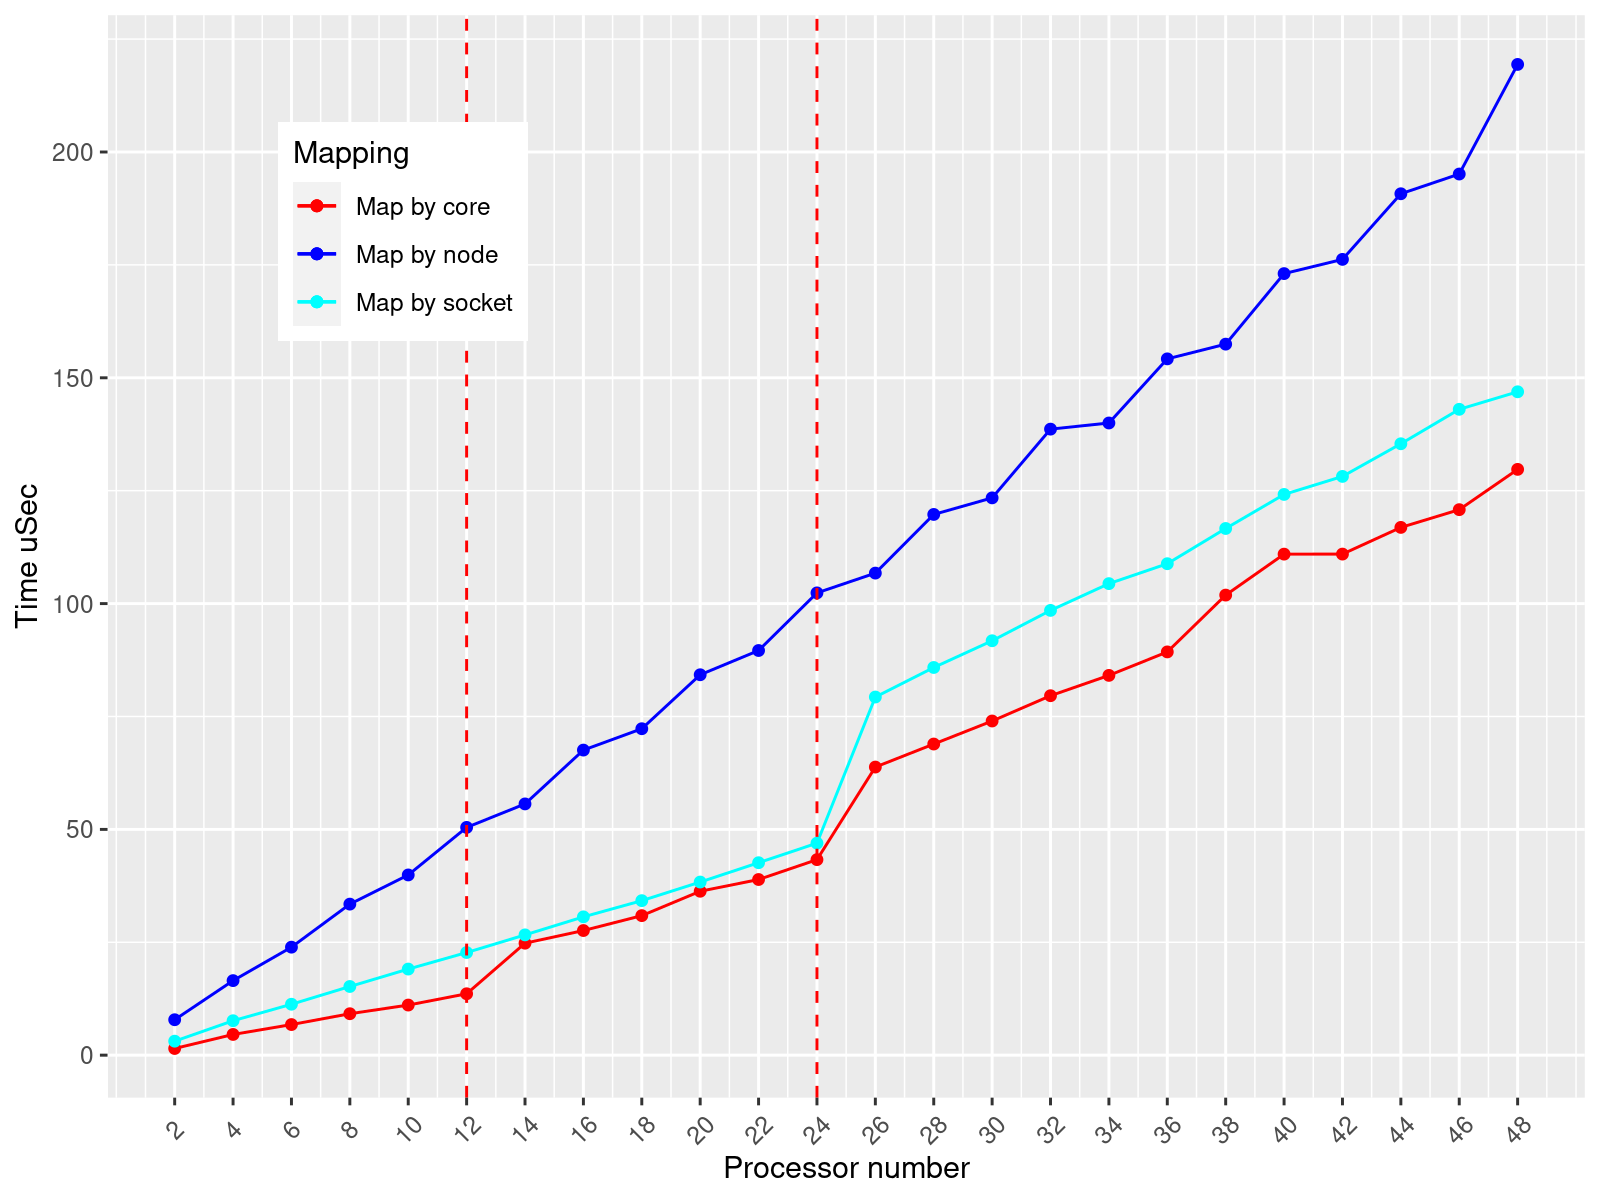
\includegraphics[width=\textwidth]{ring.png}
    \caption{The script has been run multiple times (100) on a THIN node.}
    \label{fig:ring_performance}
\end{figure}
\section{Matrix}
In memory, a 3D array can be represented as a unique linear array. The most effective way to sum it in parallel is using collective operations. The shape of the array doesn't make any difference on how the array is represented in memory. Also the virtual topology and its relative domain decomposition do not have any impact. Indeed, we can assume that the problem is not sensible to any topology, and thus is no need of communication between neighbours. The most efficient way to communicate the sum between matrices is to use \texttt{mpi\_scatterv} and \texttt{mpi\_gatherv} collective routines. \\
\\
As we can see from the table \ref{matrix_result} all the different topologies have the same behavior given the fact that we are using only collective operations. The times collected are pretty much the same except for some fluctuations in "Runtime" (caused by the matrix filling by random numbers and by the creation of virtual topology).
\begin{table}[!ht]
    \centering
    \begin{tabular}{|l|l|l|l|}
    \hline
        Distribution & Topology & Time & Nprocessor \\ \hline
        2400x100x100 & 24x1x1 & 0.63740558 & 24 \\ \hline
        2400x100x100 & 12x2x1 & 0.63056059 & 24 \\ \hline
        2400x100x100 & 6x2x2 & 0.62238741 & 24 \\ \hline
        2400x100x100 & 4x3x2 & 0.68667042 & 24 \\ \hline
        1200x200x100 & 24x1x1 & 0.68244459 & 24 \\ \hline
        1200x200x100 & 6x2x2 & 0.71415972 & 24 \\ \hline
        1200x200x100 & 4x3x2 & 0.62713907 & 24 \\ \hline
        800x300x100 & 24x1x1 & 0.63395623 & 24 \\ \hline
        800x300x100 & 12x2x1 & 0.68399210 & 24 \\ \hline
        800x300x100 & 6x2x2 & 0.67890758 & 24 \\ \hline
        800x300x100 & 4x3x2 & 0.68265990 & 24 \\ \hline
    \end{tabular}
    \caption{Time is composed by the following operations: Scattering of matrix A and matrix B, Addition of chunk of matrices and Gathering of results into matrix C}
    \label{matrix_result}
\end{table}
\\ The complete table of results is found in the folder \texttt{section\_1/build/matrix\_times\_24.csv}
\newpage
\section{MPI PingPong performance}
In this section are presented the result obtained with the \texttt{PingPong} benchmark on ORFEO. The benchmark has been ran on multiple kind of nodes and networks, and against different implementations of MPI. \\
\indent The bandwidth and the latency estimates are computed across core, socket and different nodes, combined with different protocols and hardware devices. Each of the different setup of the program has been runned 5 times and \texttt{openMPI-4.1.1} has been used. The \texttt{pml} involved in the benchmarks are \texttt{OB1} and \texttt{UCX}. The \texttt{btl} used are \texttt{tcp} and \texttt{vader}. When the measurements across nodes were perfomed also different networks with different protocols have been selected: 25 Gbit Ethernet and 100 Gbit InfiniBand.\\
\\
Mapping the processes in the same socket show often a better performance, as expected. The behaviour before asymptotic plateau is strange and shows very different performance among different implementations, the main cause of that is due to the cache. As it can be noticed in the following two graphs, the bandwidth behaviour appears strange before 16MB included. After that point, the behaviour is stable because the message size is larger than all the caches. The larger cache is \texttt{L3} with 19MB. The effect of \texttt{L2} becomes clear after 1MB, after it all implementations start loosing bandwidth. The effect of \texttt{L1} is not clearly visible from the bandwidth due to the latency. Intel InfiniBand shows poor perfomance with respect to UCX implementation, this behaviour can be explained with cache too. 
\begin{figure}[h!]
    \centering
    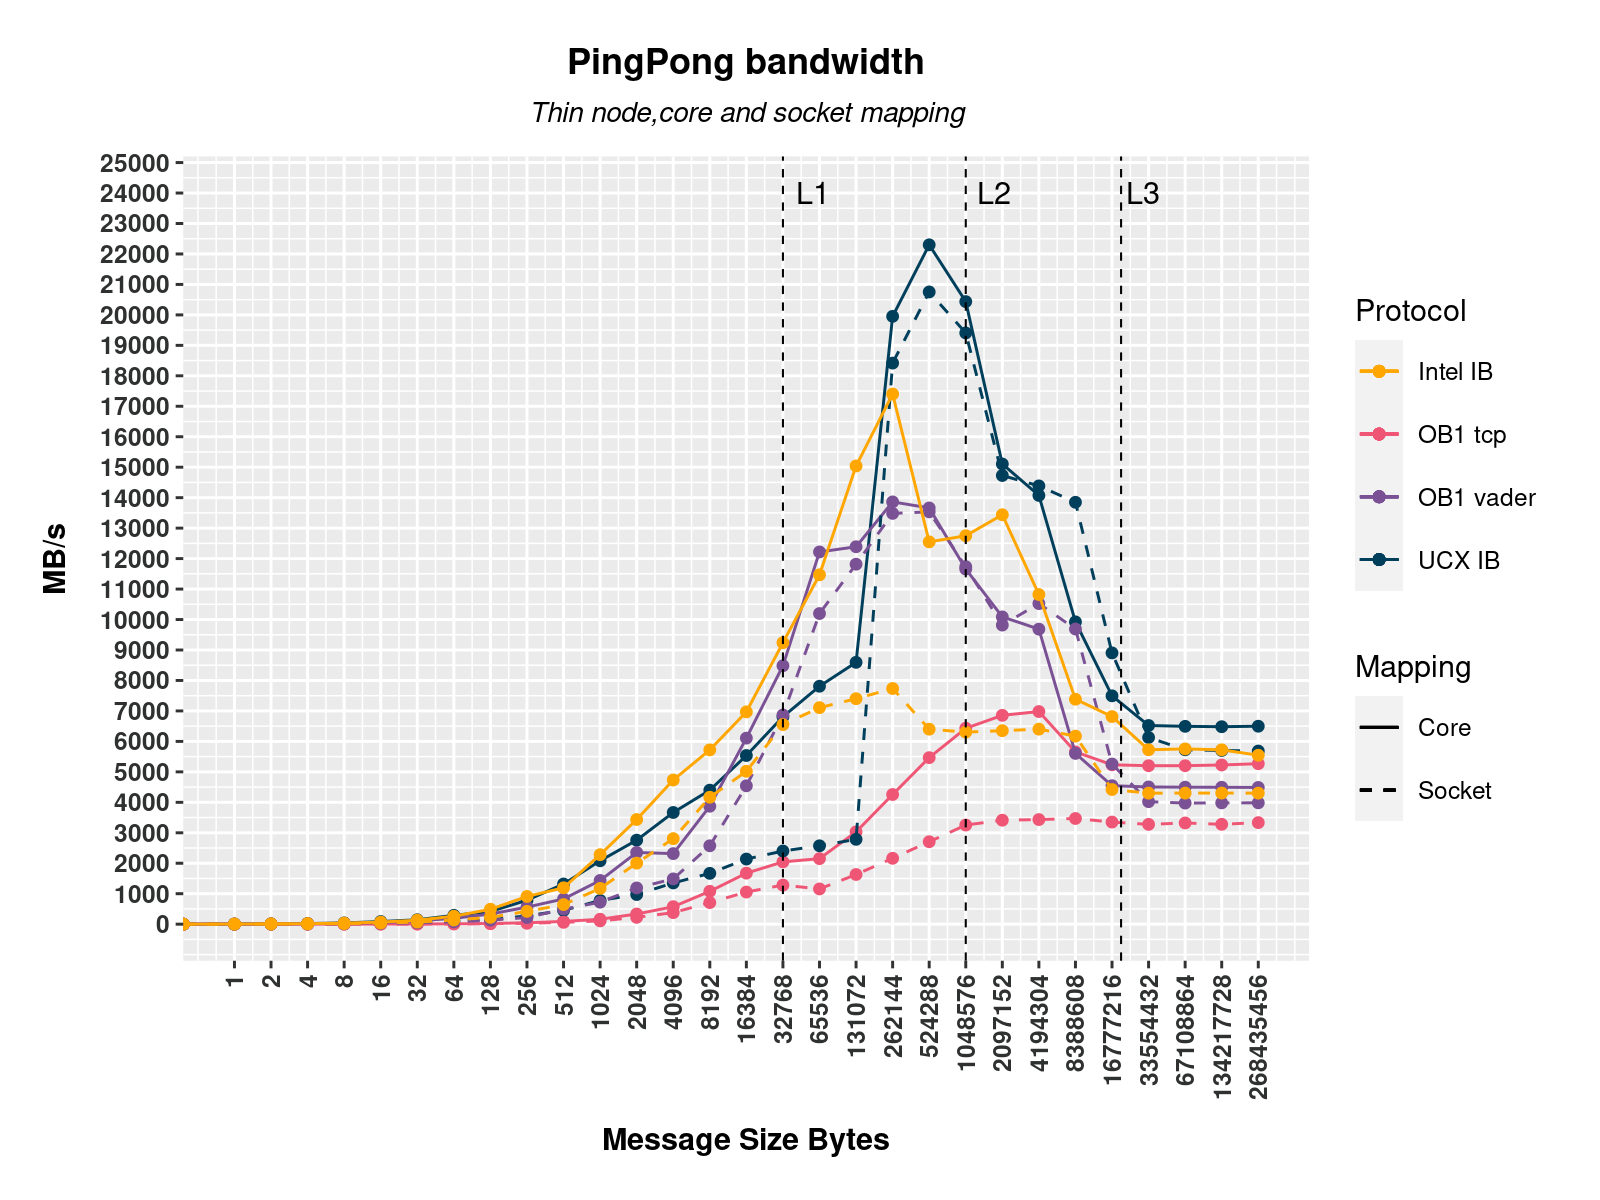
\includegraphics[width=\textwidth]{PingPongBandwidth.png}
    \label{fig:ThinPingPongBandwidth}
\end{figure}
\begin{figure}[h!]
    \centering
    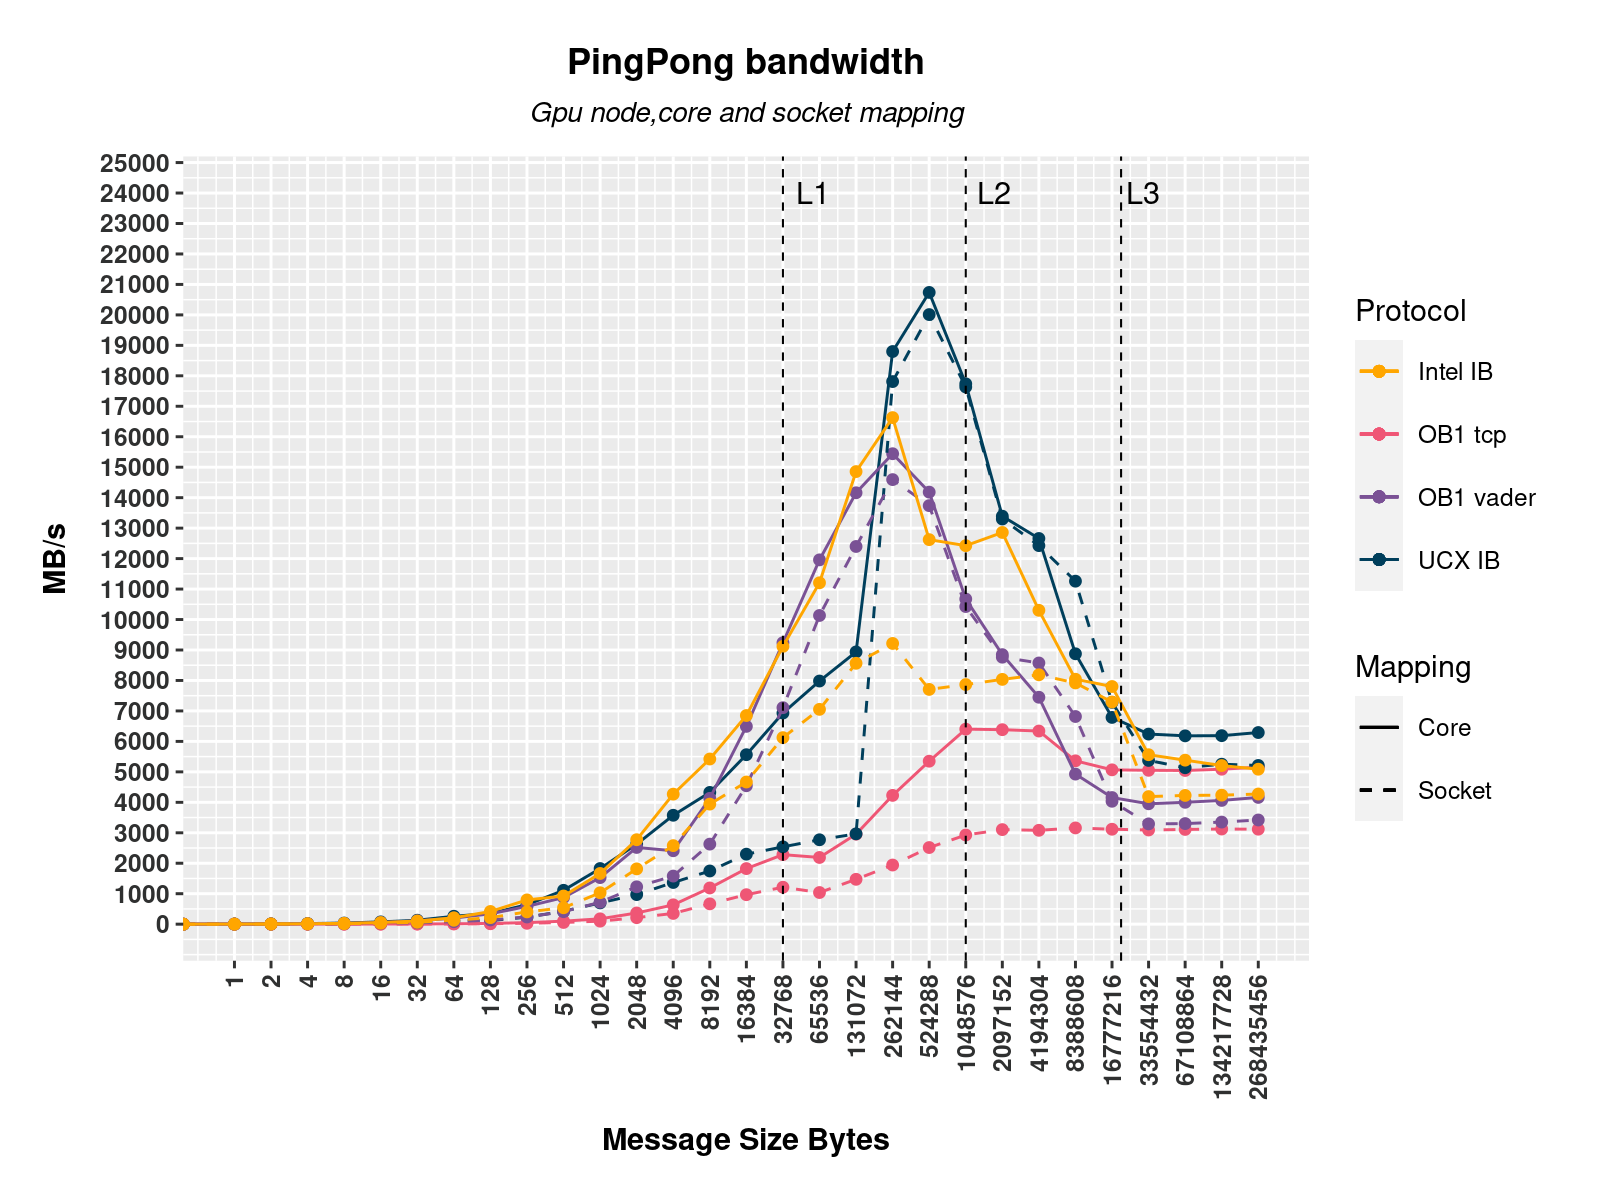
\includegraphics[width=\textwidth]{GpuPingPongBandwidth.png}
    \label{fig:GpuPingPongBandwidth}
\end{figure}
\indent From \ref{fig:ThinNodeMapping} is possible to see that with IntelMPI, UCX OpenMPI InfiniBand and UCX IB, the asymptotic bandwidth is greater than the other protocols/devices and similar to the one expected from theoretical peak.  
\begin{figure}[b!]
    \centering
    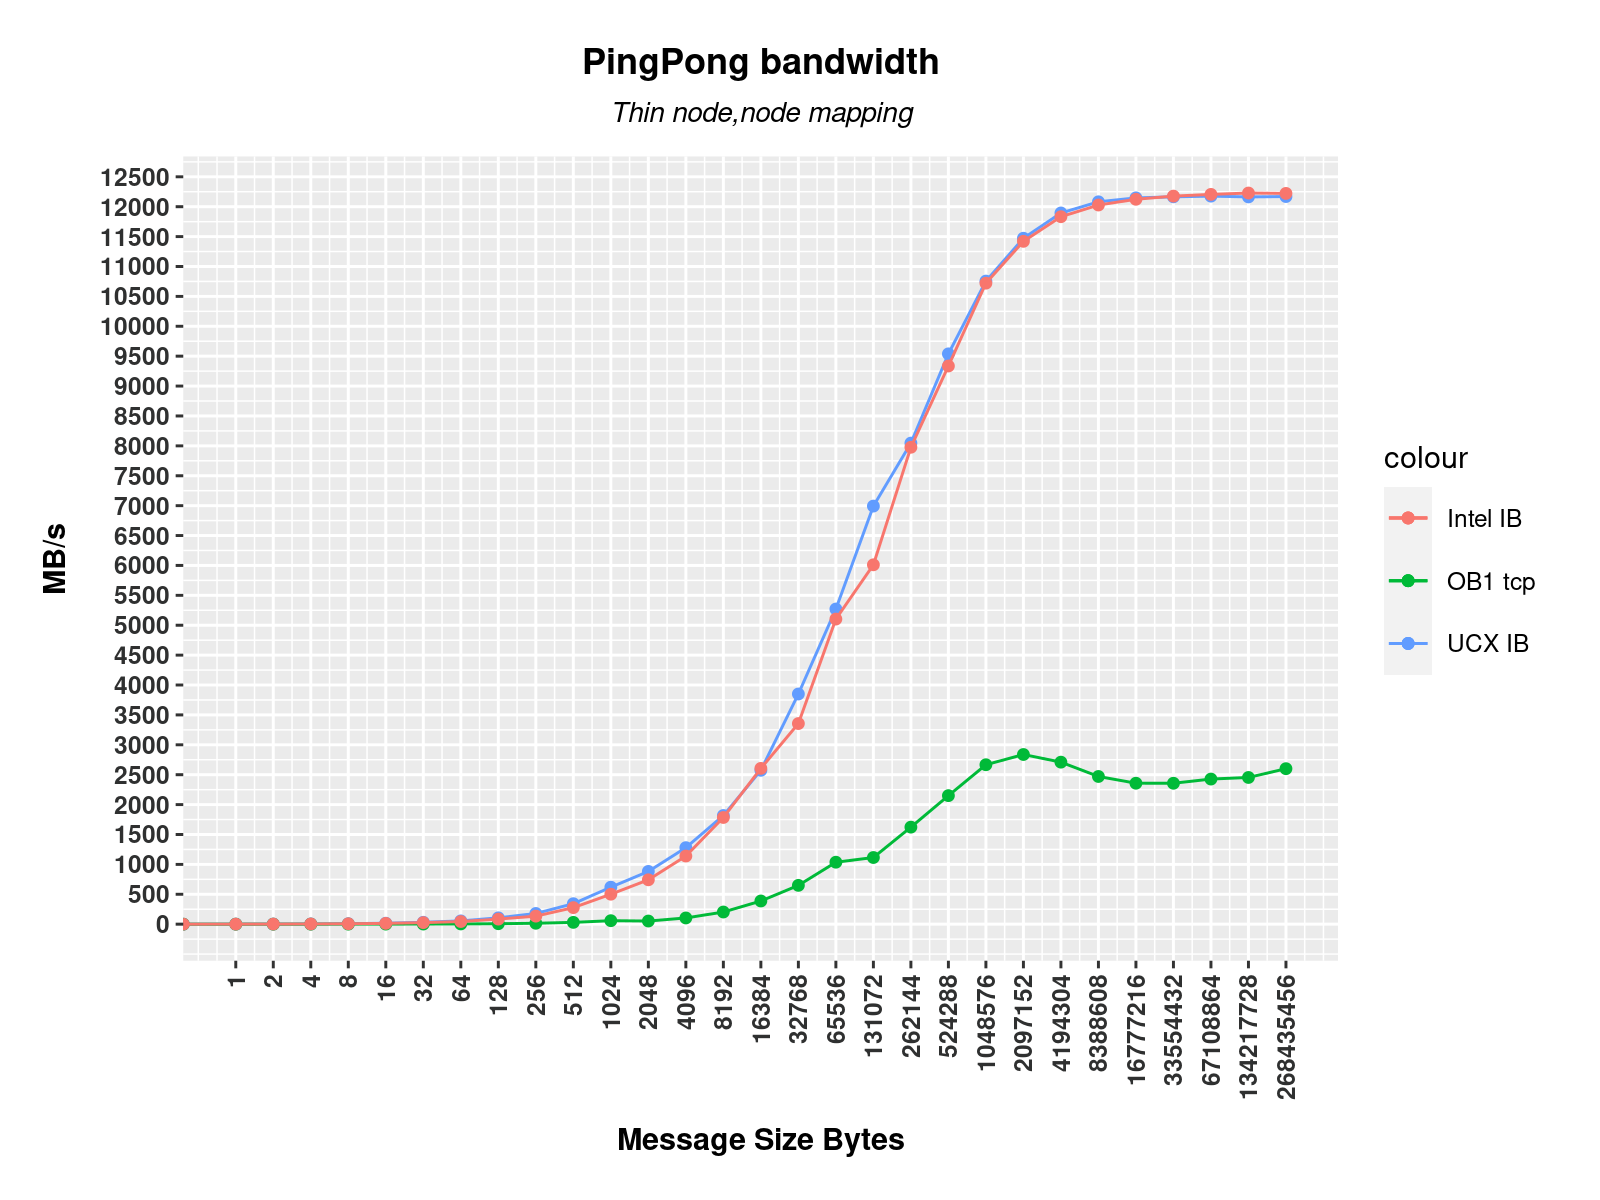
\includegraphics[width=\textwidth]{ThinNodeMapping.png}
    \caption{}
    \label{fig:ThinNodeMapping}
\end{figure}
\subsection{Differences observed between IntelMPI and OpenMPI}
It is clear that the main difference is that IntelMPI looks much more stable than OpenMPI, especially in the left region. Since the region interested by this phenomenon is the one in which the latency is dominant with respect to the bandwidth, we may assume that the two implementations communicate using different protocols with the network interface, thus encountering different costs in establishing the communication and sending the message. 
%\begin{figure}[H]
%    \centering
%    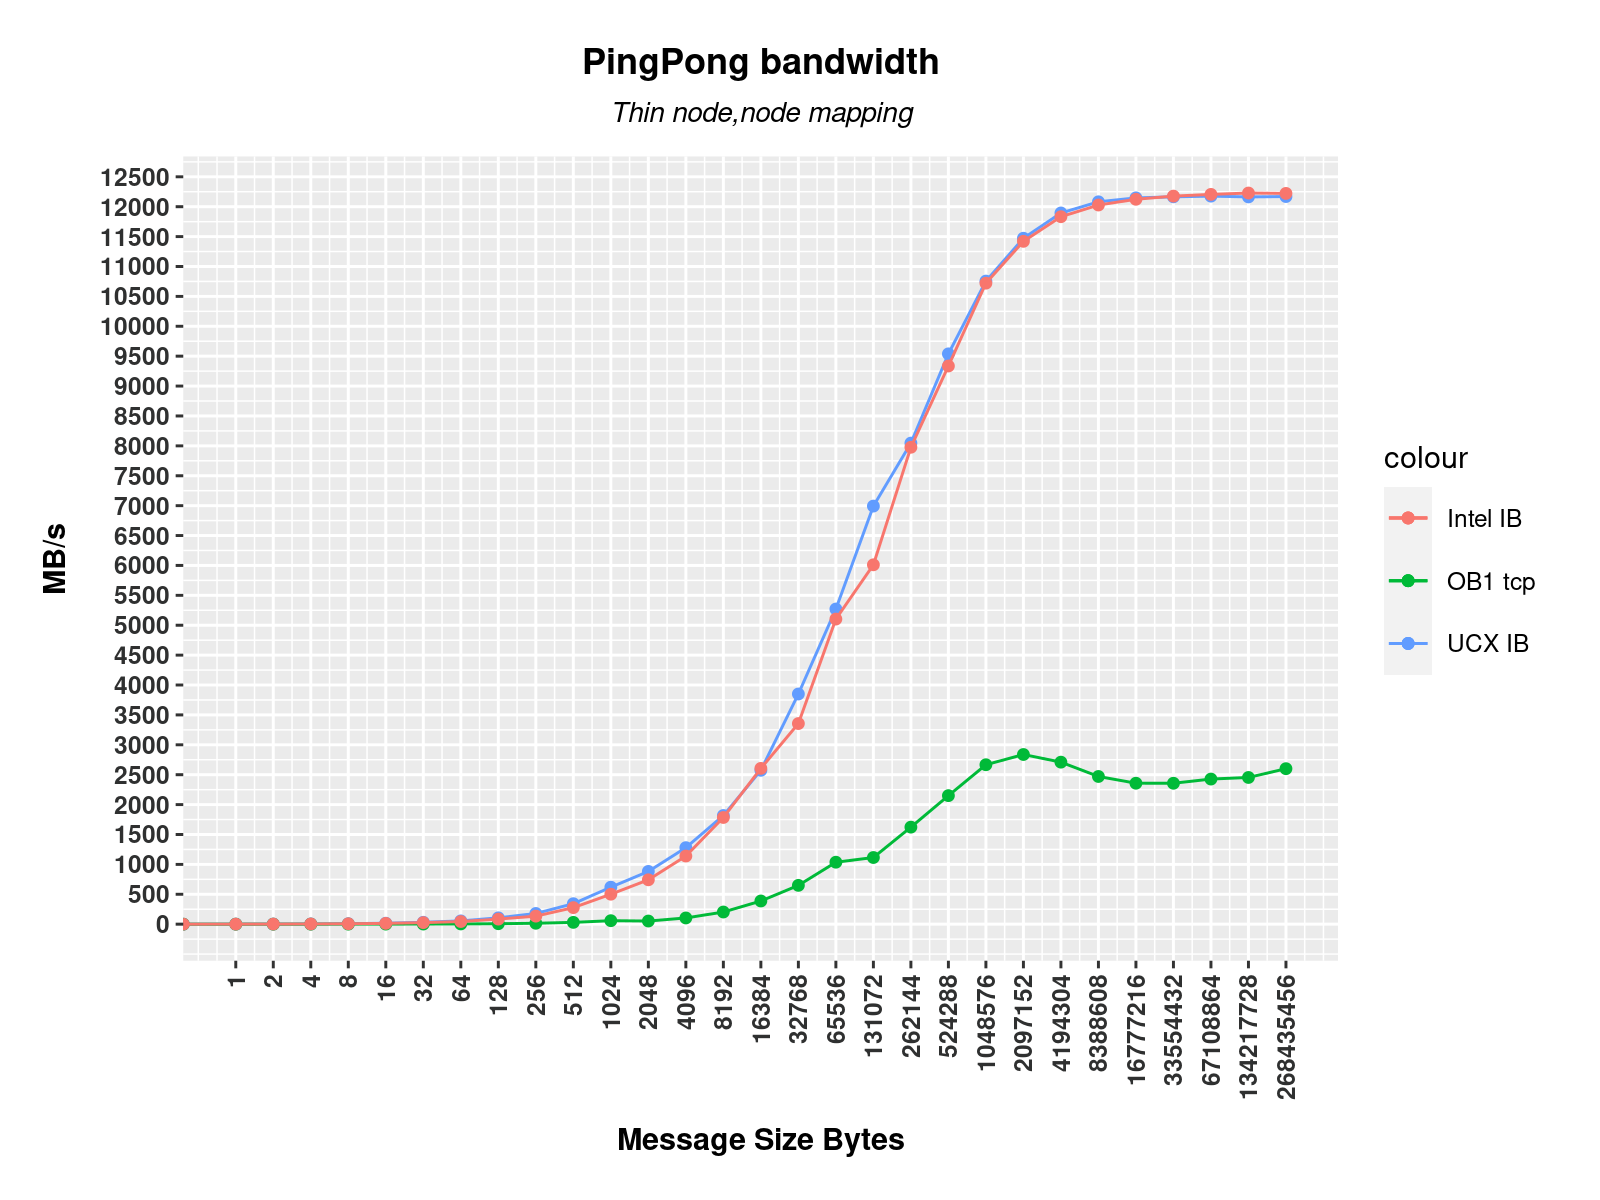
\includegraphics[width=\textwidth]{ThinNodeMapping.png}
%    \label{fig:ThinNodeMapping}
%\end{figure}
%\begin{figure}[H]
%    \centering
%    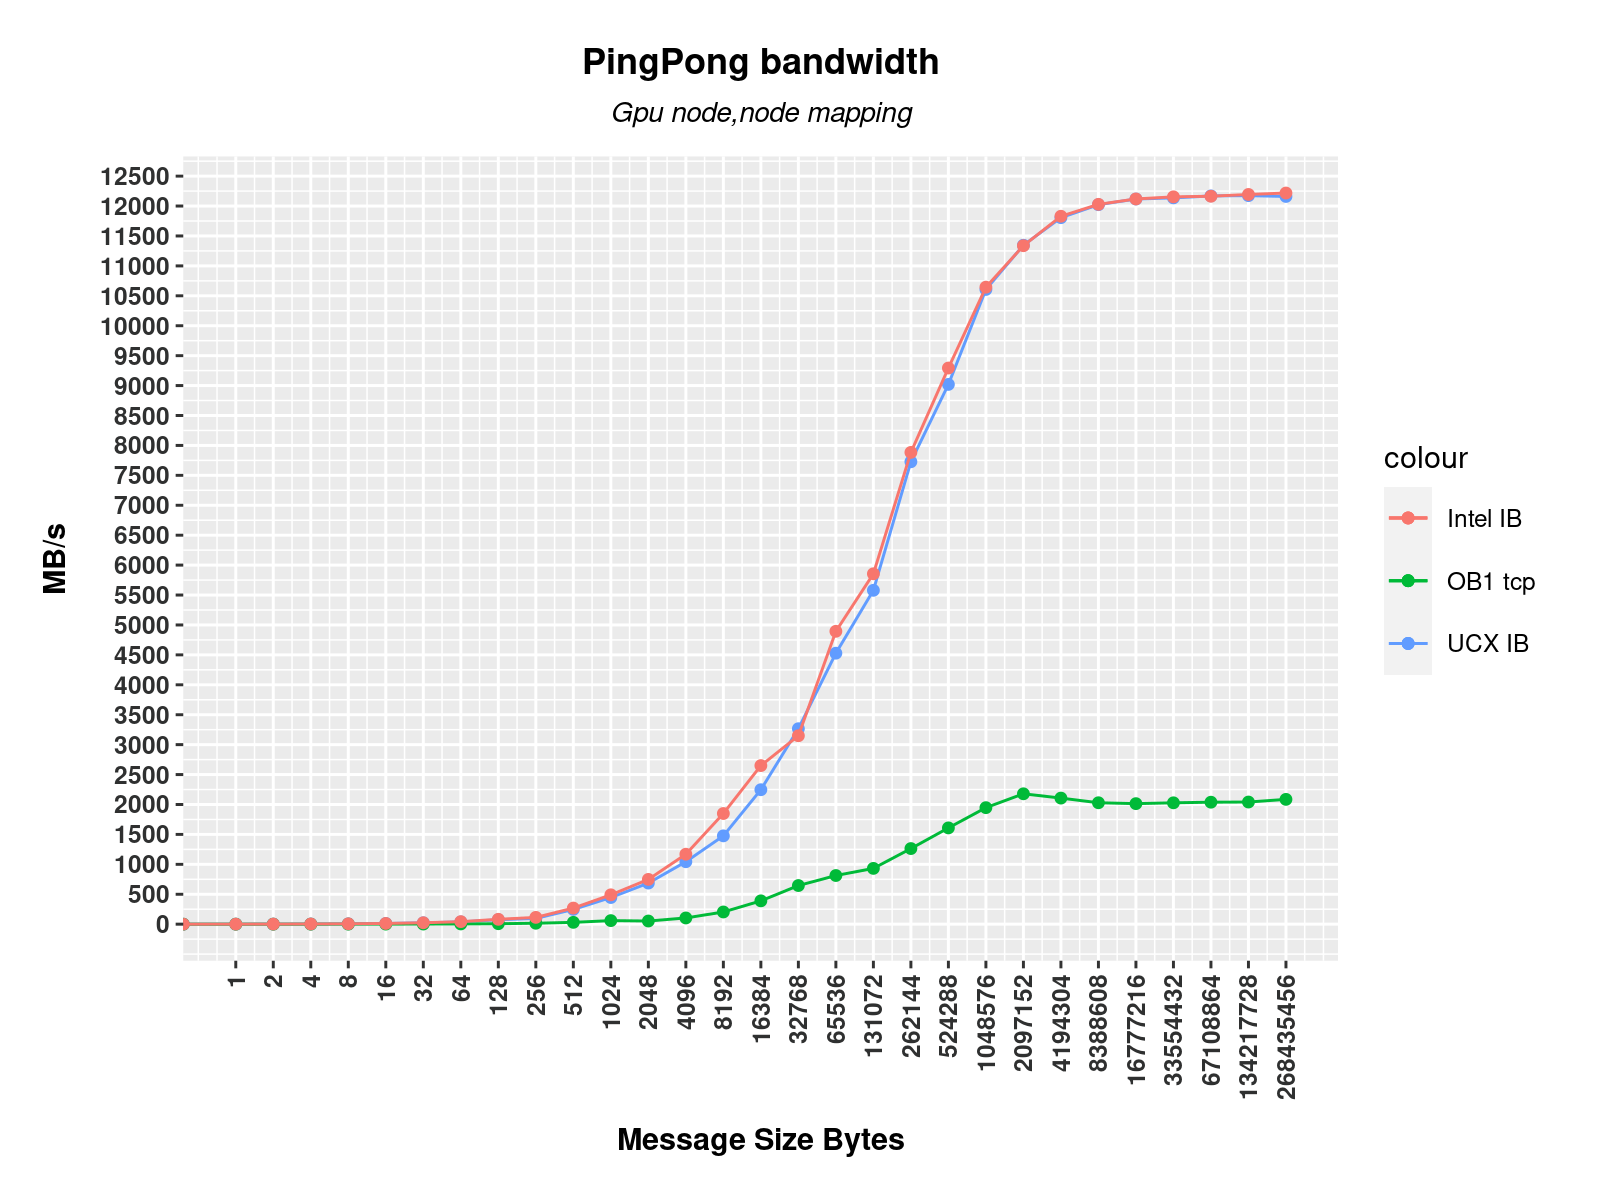
\includegraphics[width=\textwidth]{GPuNodeMapping.png}
%    \label{fig:GpuNodeMapping}
%\end{figure}
\subsection{Differences observed between Infiniband and Gigabit}
UCX with InfiniBand and Intel shows the best performance among all the configurations both in terms of latency and bandwidth. This is most likely due to the fact that Gigabit networks perform some more controls on the communication (e.g it verifies that the message arrives to the receiver), therefore message needs to pass through more layers with respect to InfiniBand networks. Also, InfiniBand employs several "tricks" to make communication faster, which likely contributes to the reduced latency. For instance when using Gigabit the user of the networks has to pre-process the message using its own computational resources. This does not happen with InfiniBand, since the pre-processing happens on a software module of the network.  
\subsection{Thin node latency and bandwidth}
\begin{table}[H]
	\centering
	\begin{tabular}{l|l|c|c}
	\toprule
	Thin node & Protocol & Latency $\mu$Sec & Bandwidth MB/$s$\\
    \midrule
    \multirow{4}*{Core mapping}	
									& UCX ib 		& $0.22$ 	& $6450.36$ \\
									& Intel ib 		& $0.24$ 	& $5702.59$ \\
									& OB1 vader 	& $0.31$ 	& $4472.75$ \\
									& OB1 tcp 		& $5.5$		& $5123.82$ \\
    \midrule
    \multirow{4}*{Socket mapping}	
									& UCX ib 		& $0.54$ 	& $5679.78$ \\
									& Intel ib 		& $0.48$ 	& $4289.15$ \\
									& OB1 vader 	& $0.72$ 	& $3954.68$ \\
									& OB1 tcp 		& $8.19$	& $3284.49$ \\   
    \midrule
    \multirow{4}*{Node mapping}	
									& UCX ib	& $1.07$ 	& $12176.39$ \\
									& Intel ib 	& $1.34$ 	& $12235.85$ \\
									& UCX ib0 	& $9.06$ 	& $2764.778$ \\
									& UCX br0 	& $15.85$ 	& $2433.241$ \\
									& OB1 tcp 	& $15.76$	& $2402.39$ \\ 
	\bottomrule
	\end{tabular}
\label{tab:ThinNodeLatency}
\end{table}
\subsection{Gpu node latency and bandwidth}
\begin{table}[H]
	\centering
	\begin{tabular}{l|l|c|c}
	\toprule
	Gpu node & Protocol & Latency $\mu$Sec & Bandwidth MB/$s$\\
    \midrule
    \multirow{4}*{Core mapping}	
									& UCX ib 		& $0.26$ 	& $6157.24$ \\
									& Intel ib 		& $0.32$ 	& $5216.97$ \\
									& OB1 vader 	& $0.30$ 	& $4030.76$ \\
									& OB1 tcp 		& $5.03$	& $5072.48$ \\
    \midrule
    \multirow{4}*{Socket mapping}	
									& UCX ib 		& $0.60$ 	& $5201.56$ \\
									& Intel ib 		& $0.53$ 	& $4209.24$ \\
									& OB1 vader 	& $0.71$ 	& $3318.39$ \\
									& OB1 tcp 		& $8.73$	& $3121.66$ \\   
	\midrule					 
    \multirow{4}*{Node mapping}	
									& UCX ib		& $1.58$ 	& $12185.46$ \\
									& Intel ib 		& $1.48$ 	& $12200.16$ \\
									& UCX ib0		& $12.94$ 	& $2432.17$ \\
									& UCX br0		& $17.82$	& $1921.84$ \\
									& OB1 tcp 		& $15.62$	& $2038.15$ \\ 
	\bottomrule
	\end{tabular}
\label{tab:GpuNodeLatency}
\end{table}
\subsection{Other observations}
GPU nodes behave like THIN nodes, and thus no difference can be seen, GPU Node is only a bit slower than THIN node. This can be due to different GPU frequency and node configuration. Cache size are the same of THIN nodes, and this cache effect are similar.
\newpage
\section{Jacobi solver}
\subsection{Performance}
To predict the performance of the Jacobi model we use the following formula:
\begin{equation}
P(L,N)=\dfrac{L^3 N}{T_s + T_c}[MLUP/s]
\end{equation}
$L$ is the size of cubic sub-domains, $T_s$ is the time for the lattice updates of a domain with size $L$ and $T_c$ is the communication time. The quantity $T_s$ can be modeled estimating the latency $\lambda$, bandwidth $B$ and messages size $C$.
\begin{equation}
T_c = \dfrac{C(L,N)}{B}+4k\lambda[s]
\end{equation}
$C(L,N)$ is the maximum bidirectional bandwidth data volume transferred over a node's network link, $k$ is the largest number of coordinate directions in which the number of processes is greater than one and $\lambda$ is the latency. The formula for $C$ is:
\begin{equation}
C = L^2 \times k \times 2 \times 8[byte]
\end{equation}
\subsection{Results}
The following tables compare the results obtained by running Jacobi with the performance model. In thin nodes, the performance $P(N,L)$ predicted from theoretical model reflect the real performance obtained from computation well. In Gpu nodes, instead there is an overestimation from the model, this could happen because hyper-threading enabled is on this node.
\subsection*{THIN node, core mapping}
$\lambda$ = $0.22$, Bandwidth = $6450.36$
\begin{table}[H]
    \centering
    \begin{tabular}{|l|l|l|l|l|l|l|l|}
    \toprule
    N 		& k 	& C[Mb] 	& Tc/s 			& MLUP/s est 	& MLUP/s real 	& MLUP/s diff  & NP(1)P(N) \\
    \midrule
    $1$ 	& $2$ 	& $46.08$ 	& $0.00714423$ 	& $112.741$ 	& $112.738$ 	&-$0.00312003$ & $1$ \\
    $4$ 	& $4$ 	& $92.16$ 	& $0.0142885$ 	& $450.755$ 	& $451.917$ 	&$1.16281$ & $0.997864$ \\
    $8$ 	& $6$ 	& $138.24$ 	& $0.0214327$ 	& $901.089$ 	& $890.34$ 		&-$10.749$ & $1.01299$ \\
    $12$ 	& $6$ 	& $138.24$ 	& $0.0214327$ 	& $1351.63$ 	& $1325.43$ 	&-$26.2079$ & $1.0207$ \\
    \bottomrule
    \end{tabular}
\end{table}
\subsection*{THIN node, socket mapping}
$\lambda$ = $0.54$, Bandwidth = $5679.78$
\begin{table}[H]
    \centering
    \begin{tabular}{|l|l|l|l|l|l|l|l|}
    \toprule
    N 		& k 	& C[Mb] 	& Tc/s 			& MLUP/s est 	& MLUP/s real 	& MLUP/s diff  & NP(1)P(N) \\
    \midrule
    $1$ 	& $2$ 	& $46.08$ 	& $0.00811407$ 	& $112.741$ 	& $112.738$ 	&$0.00401334$ & $1$ \\
    $4$ 	& $4$ 	& $92.16$ 	& $0.0162281$ 	& $450.755$ 	& $447.417$ 	&-$3.28006$ & $1.0079$ \\
    $8$ 	& $6$ 	& $138.24$ 	& $0.0243422$ 	& $901.089$ 	& $883.429$ 	&-$17.4894$ & $1.02091$ \\
    $12$ 	& $6$ 	& $138.24$ 	& $0.0243422$ 	& $1351.63$ 	& $1336.19$ 	&-$15.1886$ & $2.09478$ \\
    \bottomrule
    \end{tabular}
\end{table}
\subsection*{THIN node, node mapping}
$\lambda$ = $1.07$, Bandwidth = $12176.39$
\begin{table}[H]
    \centering
    \begin{tabular}{|l|l|l|l|l|l|l|l|}
    \toprule
    N 		& k 	& C[Mb] 	& Tc/s 			& MLUP/s est 	& MLUP/s real 	& MLUP/s diff  & NP(1)P(N) \\
    \midrule
    $1$ 	& $2$ 	& $46.08$ 	& $0.00378651$ 	& $112.766$ 	& $112.738$ 	&-$0.0278236$ & $1$ \\
    $4$ 	& $4$ 	& $92.16$ 	& $0.0113595$ 	& $1352.52$ 	& $1326.58$ 	&-$25.942$ & $1.01981$ \\
    $8$ 	& $6$ 	& $138.24$ 	& $0.0113595$ 	& $2705.04$ 	& $2627.13$ 	&-$77.913$ & $1.02991$ \\
    $12$ 	& $6$ 	& $138.24$ 	& $0.0113595$ 	& $5410.09$ 	& $5131.27$ 	&-$278.814$ & $1.0546$ \\
    \bottomrule
    \end{tabular}
\end{table}
\subsection*{GPU node, core mapping}
$\lambda$ = $0.26$, Bandwidth = $6157.24$
\begin{table}[H]
    \centering
    \begin{tabular}{|l|l|l|l|l|l|l|l|}
    \toprule
    N 		& k 	& C[Mb] 	& Tc/s 			& MLUP/s est 	& MLUP/s real 	& MLUP/s diff  & NP(1)P(N) \\
    \midrule
    $1$ 	& $2$ 	& $46.08$ 	& $0.00748439$ 	& $78.1282$ 	& $78.1421$ 	&$0.0138761$ & $1$ \\
    $4$ 	& $4$ 	& $92.16$ 	& $0.0149688$ 	& $312.407$ 	& $309.684$ 	&-$2.72303$ & $1.00931$ \\
    $8$ 	& $6$ 	& $138.24$ 	& $0.0224532$ 	& $624.603$ 	& $586.338$ 	&-$38.2651$ & $1.06617$ \\
    $12$ 	& $6$ 	& $138.24$ 	& $0.0224532$ 	& $936.905$ 	& $850.567$ 	&-$86.3376$ & $1.10245$ \\
    \bottomrule
    \end{tabular}
\end{table}
\subsection*{GPU node, socket mapping}
$\lambda$ = $0.60$, Bandwidth = $5201.56$
\begin{table}[H]
    \centering
    \begin{tabular}{|l|l|l|l|l|l|l|l|}
    \toprule
    N 		& k 	& C[Mb] 	& Tc/s 			& MLUP/s est 	& MLUP/s real 	& MLUP/s diff  & NP(1)P(N) \\
    \midrule
    $1$ 	& $2$ 	& $46.08$ 	& $0.00886008$ 	& $78.1234$ 	& $78.1421$ 	&$0.0187353$ & $1$ \\
    $4$ 	& $4$ 	& $92.16$ 	& $0.0177202$ 	& $312.368$ 	& $311.43$ 		&-$0.938776$ & $1.00366$ \\
    $8$ 	& $6$ 	& $138.24$ 	& $0.0265802$ 	& $624.487$ 	& $611.262$ 	&-$13.2245$ & $1.0227$ \\
    $12$ 	& $6$ 	& $138.24$ 	& $0.0265802$ 	& $936.73$ 		& $899.664$ 	&-$37.066$ & $1.04228$ \\
    \bottomrule
    \end{tabular}
\end{table}
\subsection*{GPU node, node mapping}
$\lambda$ = $1.58$, Bandwidth = $12185.46$
\begin{table}[H]
    \centering
    \begin{tabular}{|l|l|l|l|l|l|l|l|}
    \toprule
    N 		& k 	& C[Mb] 	& Tc/s 			& MLUP/s est 	& MLUP/s real 	& MLUP/s diff  & NP(1)P(N) \\
    \midrule
    $1$ 	& $2$ 	& $46.08$ 	& $0.00378472$ 	& $78.1413$ 	& $78.1421$ 	&$0.000805104$ & $1$ \\
    $4$ 	& $4$ 	& $92.16$ 	& $0.0113541$ 	& $937.375$ 	& $897.053$ 		&-$40.3223$ & $1.04532$ \\
    $8$ 	& $6$ 	& $138.24$ 	& $0.0113541$ 	& $1874.75$ 	& $1686.53$ 	&-$188.224$ & $1.112$ \\
    $12$ 	& $6$ 	& $138.24$ 	& $0.0113541$ 	& $3749.5$ 		& $2488.66$ 	&-$1260.83$ & $1.50716$ \\
    \bottomrule
    \end{tabular}
\end{table}
The biggest difference between model and data is the communication time. In fact, the time $T_c$ predicted from the model is hundred time smaller then the observed one. However, the simple model used is good enough to predict the performance of the program. 
\end{document}
